%%===========================================================%%
%%                                                           %%
%%              DEAD MATERIAL IN FRONT OF TPC                %%
%%                                                           %%
%%===========================================================%%


\newcommand{\itemm}{\item\hspace*{-5pt}.\hspace*{-1pt}~}

\chapter{Dead material in front of TPC}\label{chap:deadMaterial}

Particle detected and reconstructed in the TPC must first pass through the detector material standing in between the accelerator vacuum and TPC gas. This affects track reconstruction efficiency, as the particle may interact with that material - in worst case inelastically, and induce secondary particles thus lower reconstruction efficiency. Accuracy of modeling of the detector material in the STAR simulation, especially in run 15 with the HFT installed, influences systematic error e.g. on the TPC track reconstruction efficiency. In this section the density of secondary vertices is compared between the data and embedded MC. The density of secondary vertices is directly propotional to the amount of the material in given volume, hence any discrepancy between secondary vertex distribution in the data and MC can be a hint for innacuracies of the STAR simulation which should be accordingly covered by the systematic uncertainties. It should be stressed that this analysis is not aimed to tune the material budget in the STAR simulation, as there are much better data for this than high-luminosity proton-proton collisions from run 15. The aim of presented study is to obtain reasonable estimate of the component of systematic uncertainty of the TPC track reconstruction effciency related to the error on the amount and distribution of inactive material.

%---------------------------%   
\begin{figure}[b!]\vspace{-10pt}
\centering
\parbox{0.4725\textwidth}{
  \centering
  \begin{subfigure}[b]{\linewidth}
                \subcaptionbox{\label{fig:multDataVsMC}}{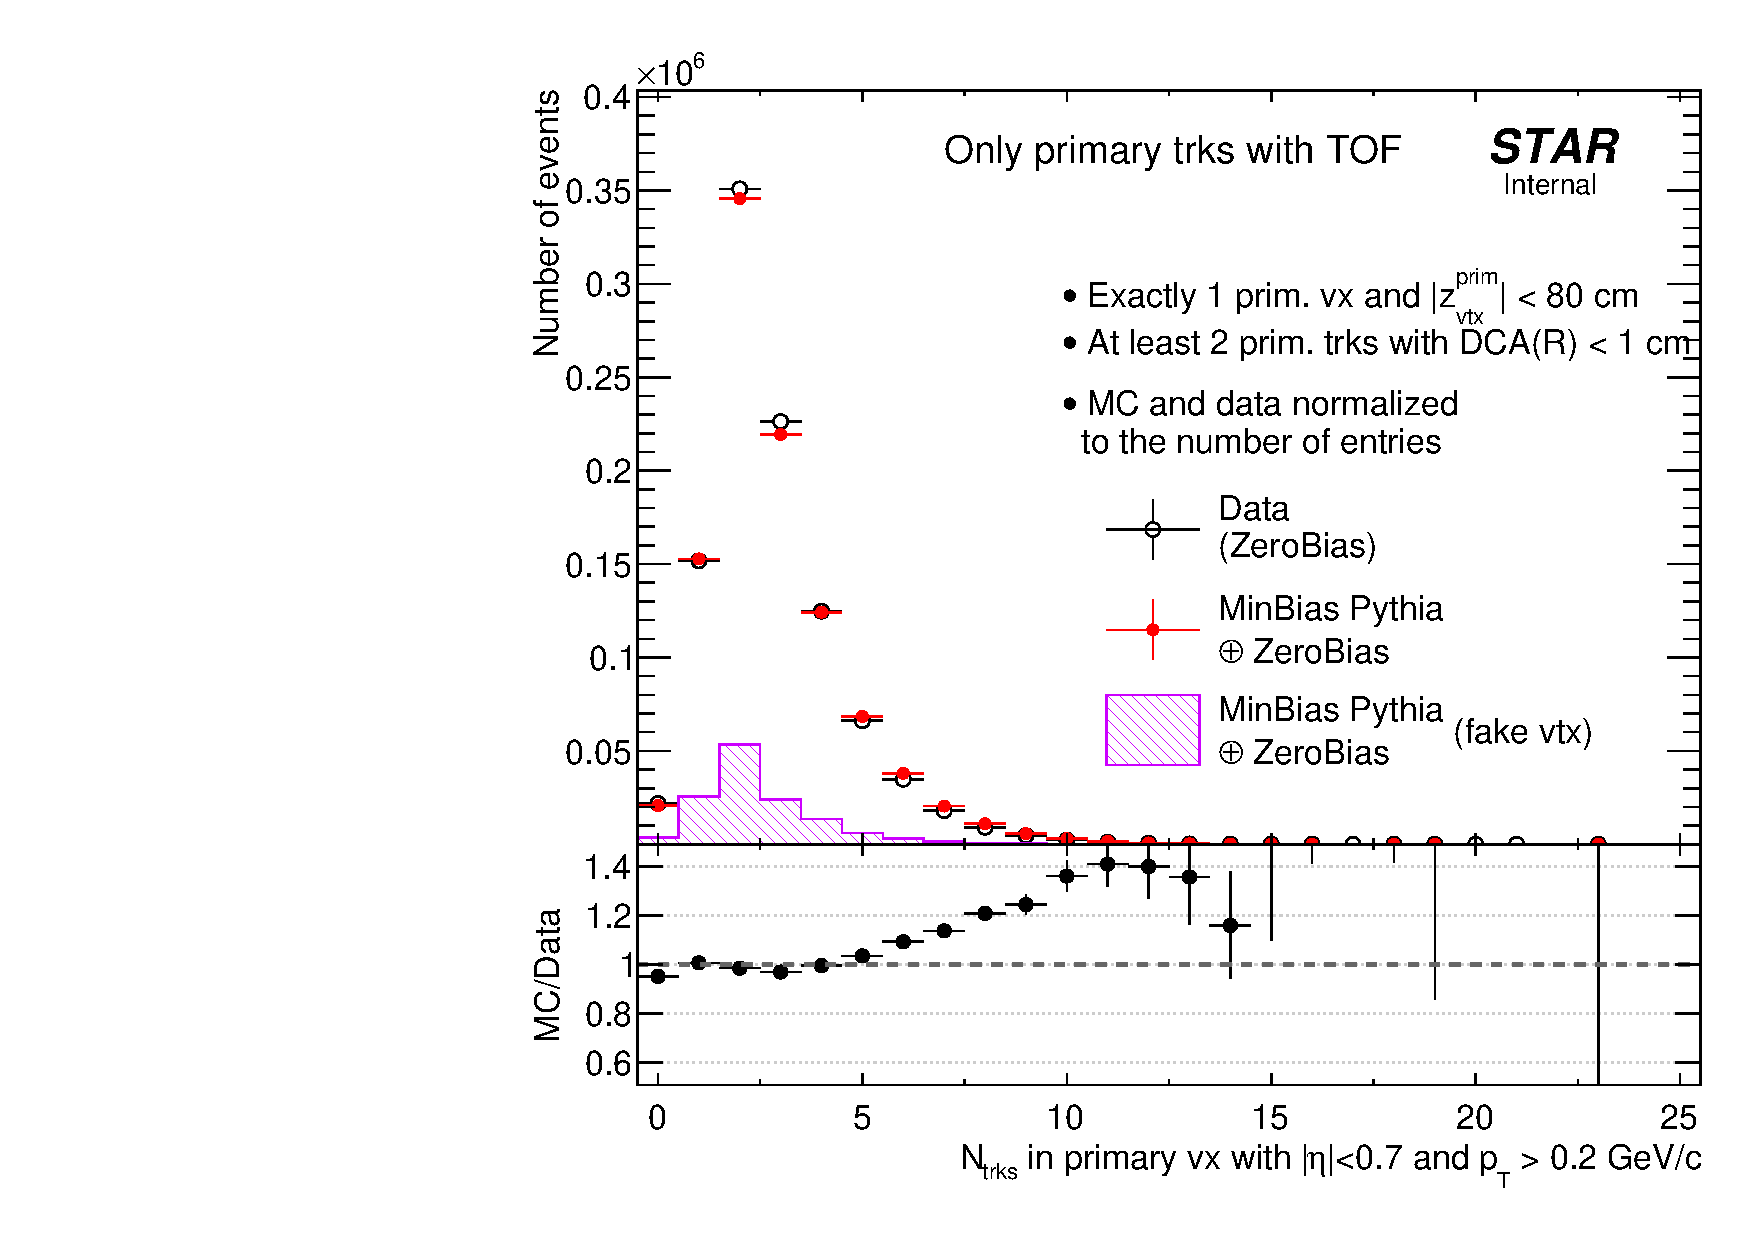
\includegraphics[width=\linewidth]{graphics/deadMaterial/NTracksPrimary_SelectedEvents_EtaPtCut_DataVsMC.pdf}}
  \end{subfigure}\\
  \begin{subfigure}[b]{\linewidth}\addtocounter{subfigure}{1}
                \subcaptionbox{\label{fig:etaDataVsMC}}{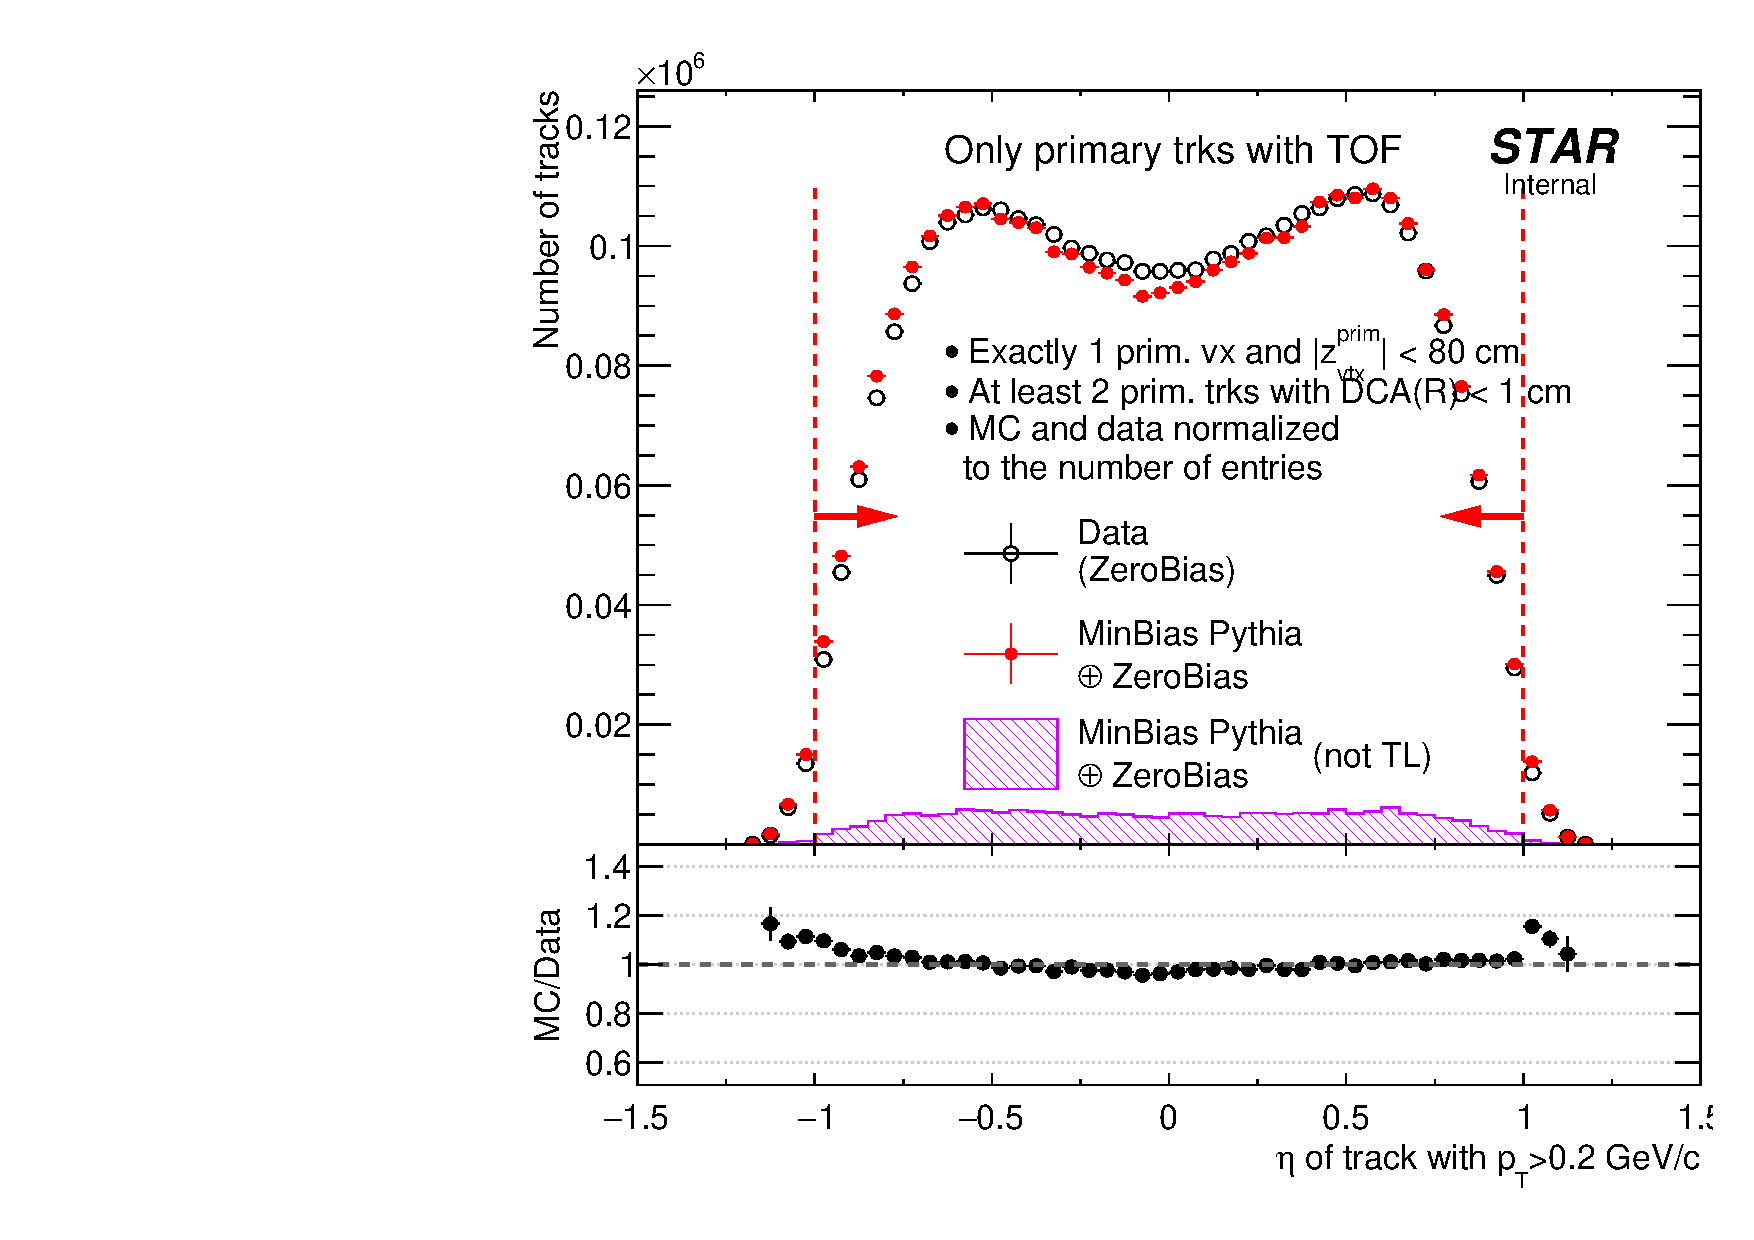
\includegraphics[width=\linewidth]{graphics/deadMaterial/TrackEtaPrimary_SelectedEvents_DataVsMC.pdf}}
  \end{subfigure}
}%
\quad\quad%
\parbox{0.4725\textwidth}{
  \centering
  \begin{subfigure}[b]{\linewidth}\addtocounter{subfigure}{-2}
                \subcaptionbox{\label{fig:ptDataVsMC}}{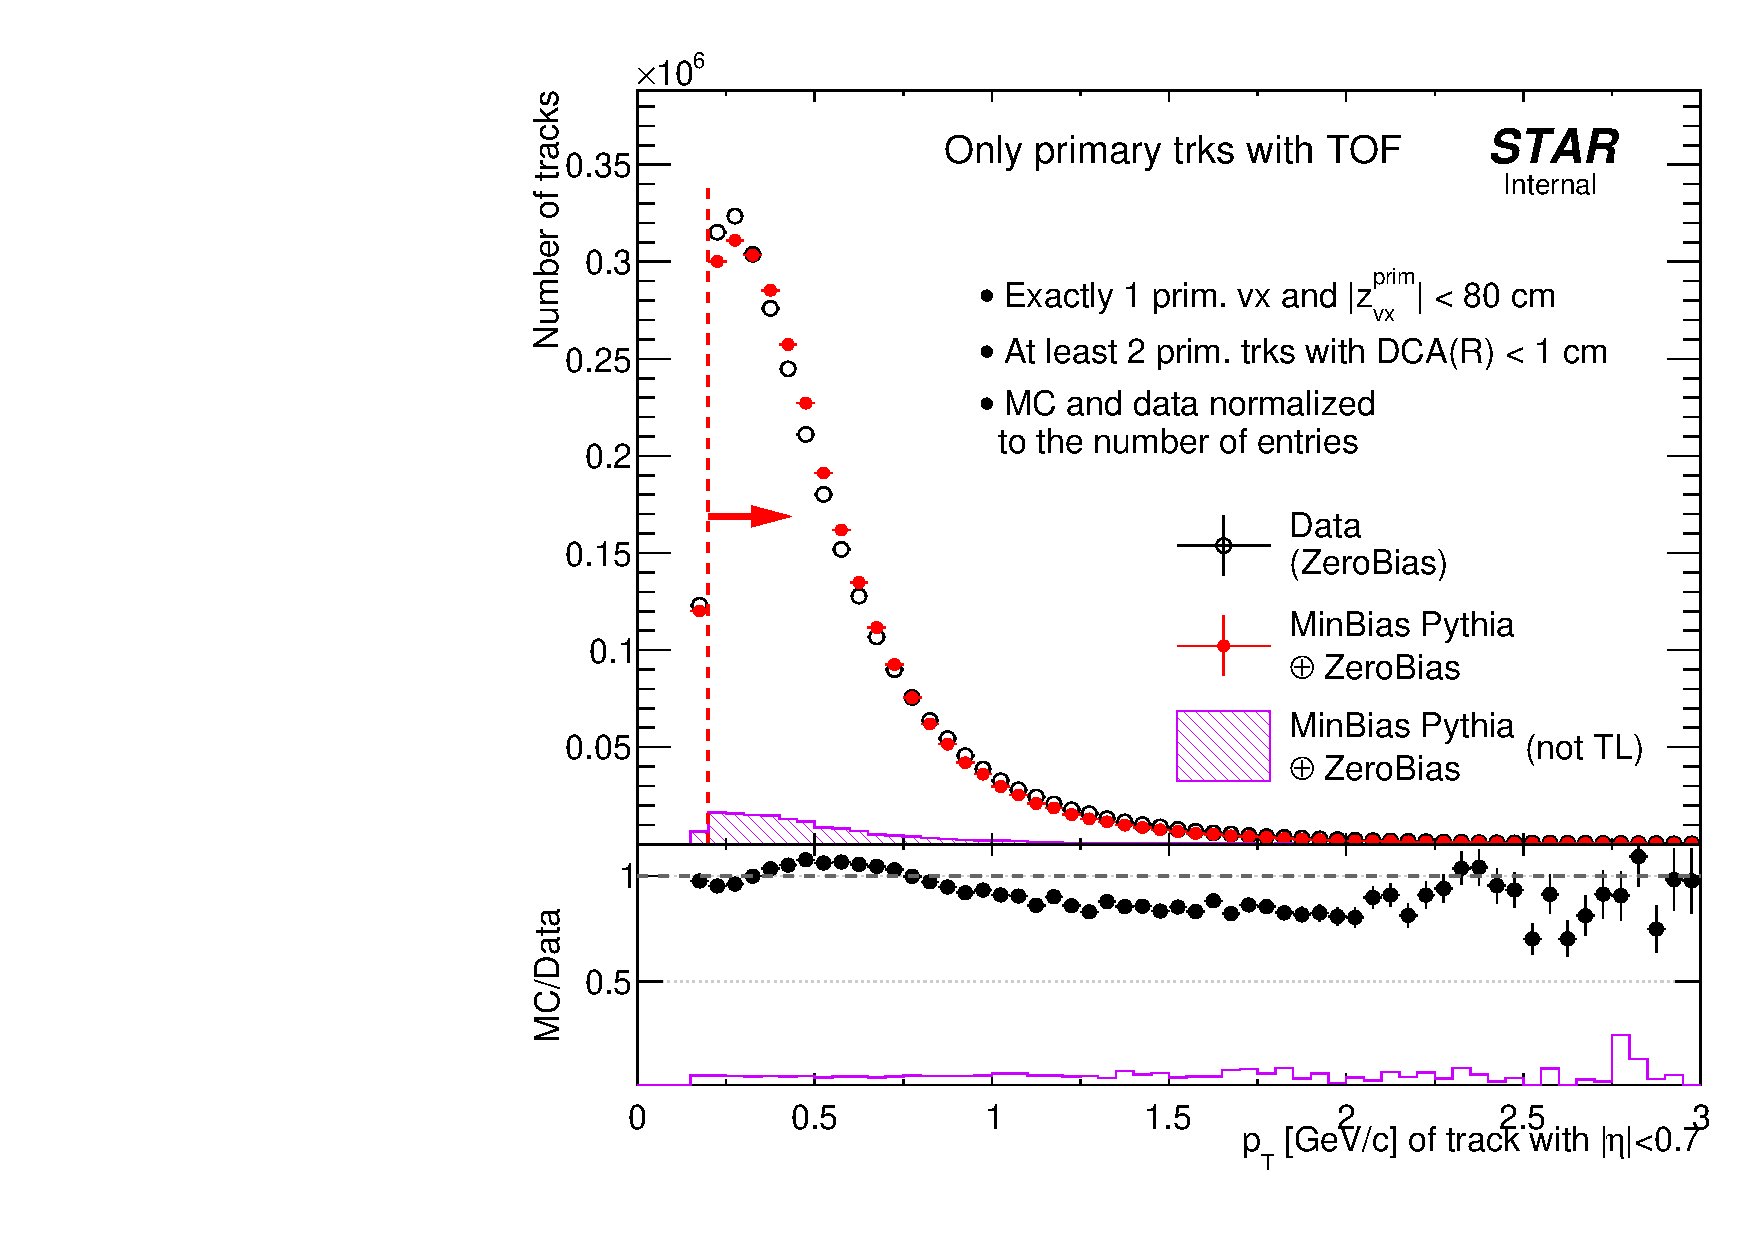
\includegraphics[width=\linewidth]{graphics/deadMaterial/TrackPtPrimary_SelectedEvents_DataVsMC.pdf}}
  \end{subfigure}\\
  \begin{minipage}[t][1.042\linewidth][t]{\linewidth}\vspace{10pt}
    \caption[Comparison of primary track multiplicity, $p_{T}$ and $\eta$ distribution in zero-bias data and embedded MC (minimum-bias).]%
    {Comparison of primary track multiplicity~(\ref{fig:multDataVsMC}), $p_{T}$~(\ref{fig:ptDataVsMC}) and $\eta$~(\ref{fig:etaDataVsMC}) distribution in zero-bias data and minimum-bias MC embedded into zero-bias triggers. In all subfigures MC histogram is normalized to have the same integral as the data histogram. Violet hashed histogram in Fig.~\ref{fig:multDataVsMC} represents the fake vertices defined as vertices of which less than a half of constituent tracks is matched to true-level particles. Violet hashed histogram in Fig.~\ref{fig:ptDataVsMC} and~\ref{fig:etaDataVsMC} represents tracks not matched to true-level particles. Bottom pads in each figure show the ratio between MC and data as black points, and the ratio between fake (violet histogram) and all MC entries (red points) as a violet line. Red dashed lines and arrows indicate range of tracks required in selection of events for the secondary vertex analysis.}\label{fig:deadMatDataVsMC}
  \end{minipage}
}\vspace{-20pt}%
\end{figure}
%---------------------------

Analysis of the distribution of secondary vertices was performed using both zero-bias (ZB) data and minimum-bias MC (Pythia) embedded into zero-bias triggers. Because of insufficient statistics of the ZB data, for the purpose of analysis presented in this section both standard ZB data sample (from ZB triggers in st\_rp stream) and the subsample of RP\_CP triggers (see Ref.~\cite{onlineRpTriggersMonitoring} for trigger details) with identified elastic proton-proton scattering events using loose RP track selection were used. The latter subsample is in good approximation a ZB sample in terms of central detector, as it was triggerd only by the east and west coincidence of Roman Pots - any particle present in the TPC and TOF is predominantly a product of pile-up interaction. In all plots and later in the text we refer to this merged sample as ZB data sample. 

Analysis started with the following selection of events:\vspace{-5pt}
\begin{enumerate}
 \item Exactly 1 reconstructed primary vertex (with tracks matched to hits in TOF; beamline constraint was used in reconstruction therefore primary vertices lie on the beamline and tracks associated with them have global DCA ($d_{0}$) not larger than $\approx$ 1.5~cm),\vspace{-5pt}
 \item $|z_{vx}|<80$~cm\vspace{-5pt},
 \item $\geq$2 prim. TOF tracks with:~~~DCA(R)~$<$~1~cm,~~~$|\eta|<1$,~~~$p_{T}>0.2~\text{GeV}/c$,~~~$N_{\textrm{hits}}^{\textrm{fit}}\geq25$,~~~$N_{\textrm{hits}}^{\textrm{dE/dx}}\geq15$.%,~~~~~~~~$N_{\textrm{hits}}^{\textrm{fit}}/N_{\textrm{hits}}^{\textrm{poss}}\geq0.52$.
\end{enumerate}%
The aim of above criteria was to select pile-up-free events with well defined vertex. Cut on $z$-vertex is identical to one used in physics analyses. Figure~\ref{fig:deadMatDataVsMC} shows comparison of quantities characterizing an event. In general a moderate agreement between MC and data can be observed, considered sufficient for trustworthy result of described analysis.
%---------------------------
\begin{figure}[b!]\vspace{-19pt}
\centering
\parbox{0.4725\textwidth}{
  \centering
  \begin{subfigure}[b]{\linewidth}
                \subcaptionbox{\label{fig:D0yVsD0xGlobalTofTrks_Data}}{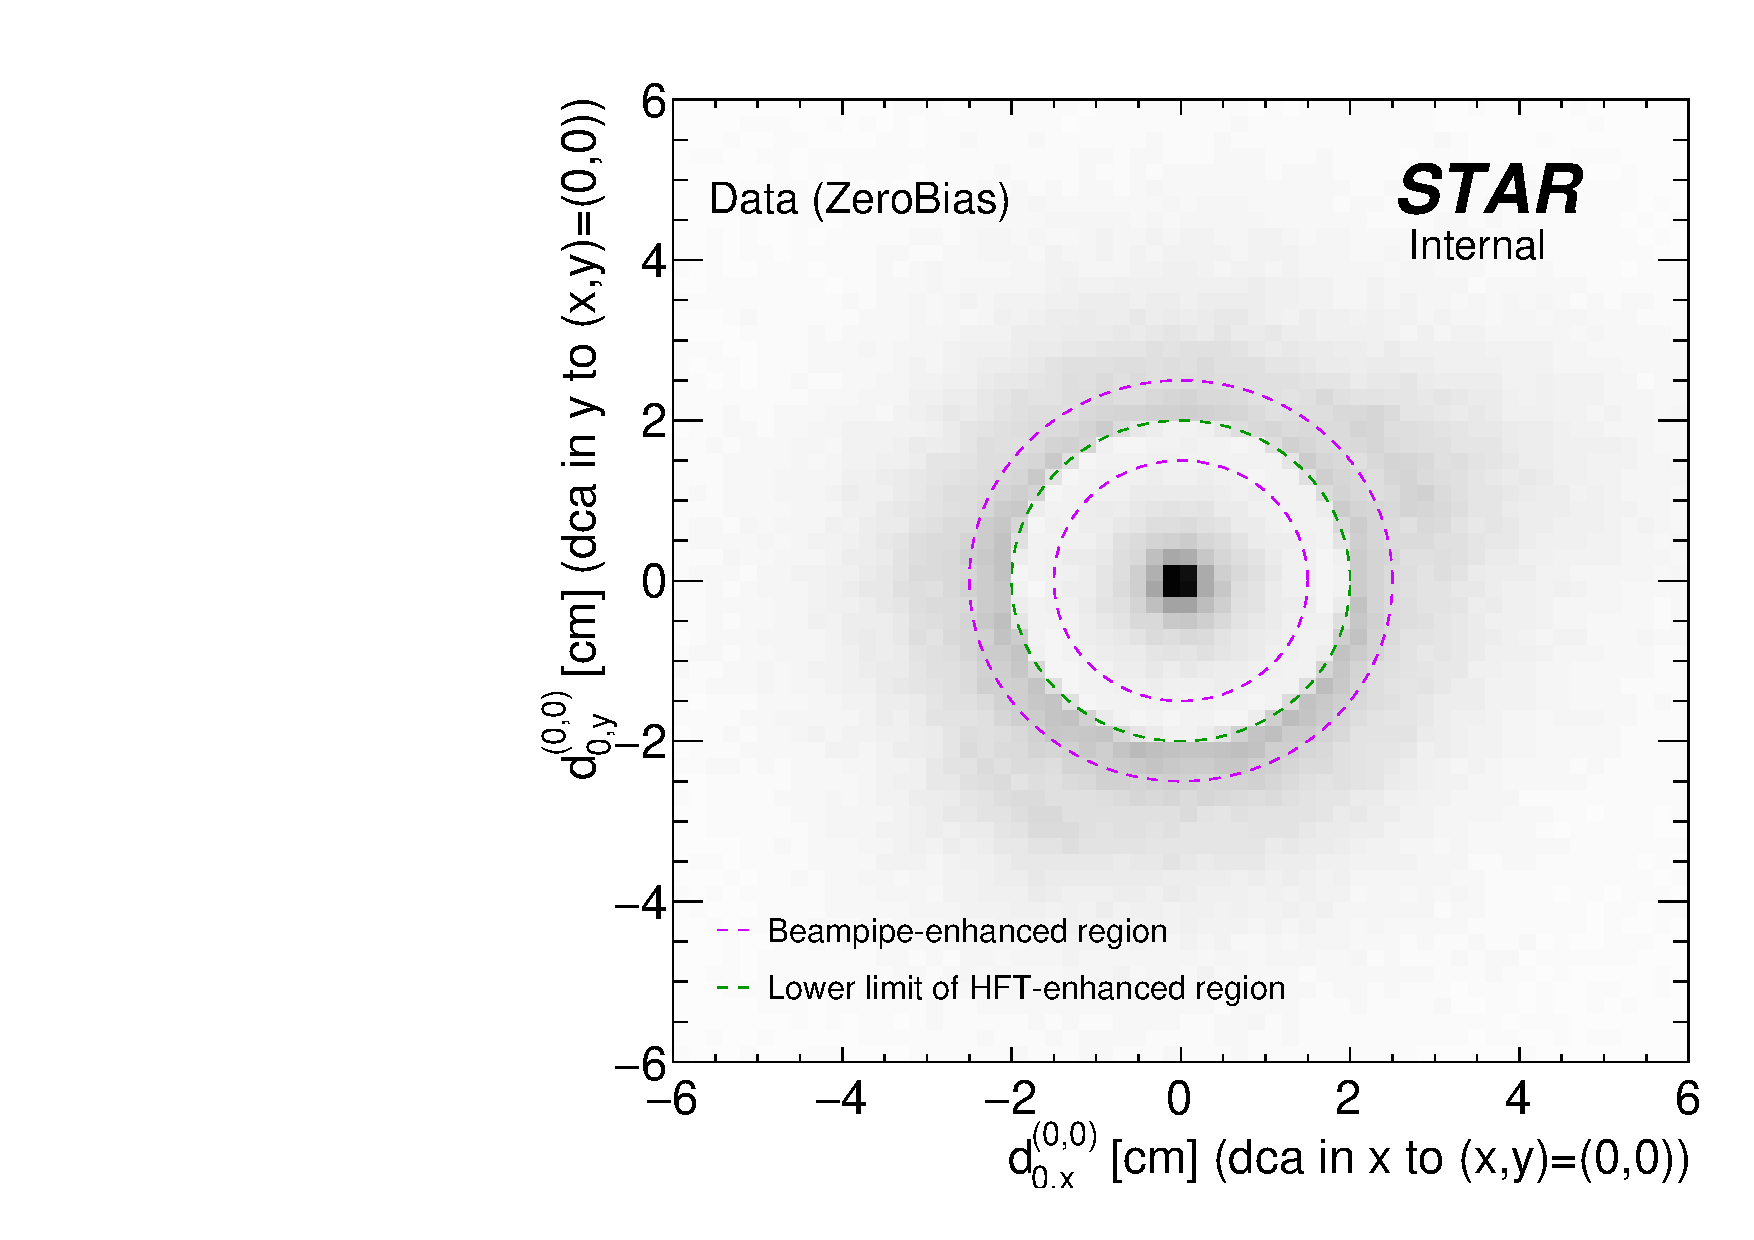
\includegraphics[width=\linewidth,page=1]{graphics/deadMaterial/D0yVsD0xGlobalTofTrks_DataVsMC.pdf}}
  \end{subfigure}\\
  \begin{subfigure}[b]{\linewidth}\addtocounter{subfigure}{1}
                \subcaptionbox{\label{fig:D0GlobalTofTrks_DataVsMC}}{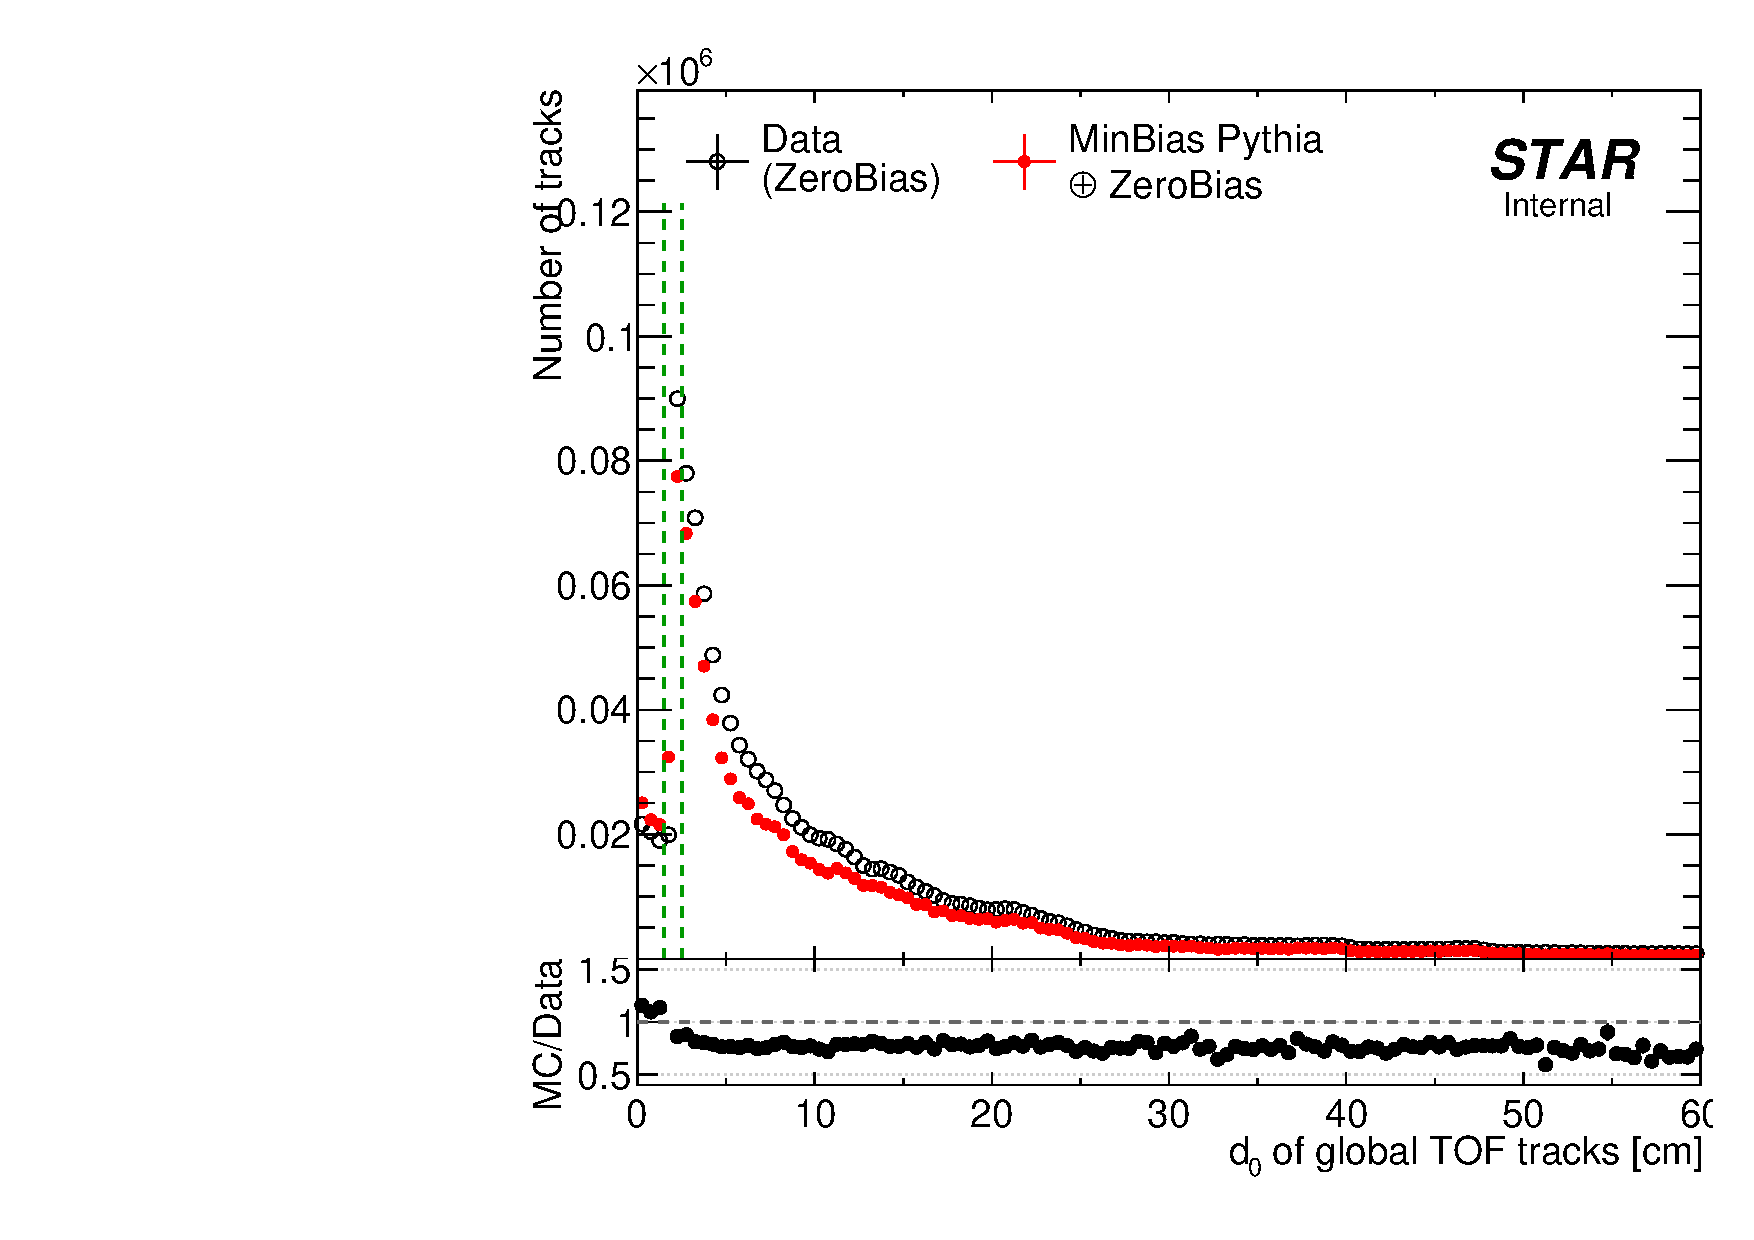
\includegraphics[width=\linewidth]{graphics/deadMaterial/D0GlobalTofTrks_DataVsMC.pdf}}
  \end{subfigure}
}%
\quad\quad%
\parbox{0.4725\textwidth}{
  \centering
  \begin{subfigure}[b]{\linewidth}\addtocounter{subfigure}{-2}
                \subcaptionbox{\label{fig:D0yVsD0xGlobalTofTrks_MC}}{\includegraphics[width=\linewidth,page=2]{graphics/deadMaterial/D0yVsD0xGlobalTofTrks_DataVsMC.pdf}}
  \end{subfigure}\\
  \begin{minipage}[t][1.042\linewidth][t]{\linewidth}\vspace{10pt}
    \caption[Comparison of $d_{0}^{(0,0)}$ distribution of global TPC tracks matched with TOF in zero-bias data and embedded MC (minimum-bias).]{Two-dimensional $d_{0}^{(0,0)}$ distribution of global TPC tracks matched with TOF in zero-bias data (\ref{fig:D0yVsD0xGlobalTofTrks_Data}) and embedded minimum-bias MC (\ref{fig:D0yVsD0xGlobalTofTrks_MC}), and comparison of their radial projection in wider range of $d_{0}^{(0,0)}$ (\ref{fig:D0GlobalTofTrks_DataVsMC}). Distributions were normalized to the number of primary tracks, according to Eq.~\eqref{eq:mcNormDeadMat}. Red dashed lines and arrow indicate limit of $d_{0}^{(0,0)}$ of tracks accepted for the secondary vertex analyses (limit equals 2~cm). In all subfigures there are only entries from global tracks not associated with the primary tracks. Even with relatively low pointing resolution of the TPC tracks ($\sim$1~cm) one can recognize structures which can be atrributed the beampipe starting at $d_{0}^{(0,0)}=2$~cm, and HFT elements at about 8~cm, 11~cm, 14~cm and 22~cm.}\label{fig:deadMatDataVsMC2}
  \end{minipage}
}\vspace{-30pt}%
\end{figure}
%---------------------------

As a next step the TPC tracks were selected for the search and reconstruction of secondary vertices. The requirements were as follows:\vspace{-5pt}
\begin{enumerate}
  \item Global TPC tracks matched with TOF not associated with any primary TPC track,\vspace{-8pt}
  \item $|\eta|<0.7$,~~~~~~~~$p_{T}>0.2~\text{GeV}/c$,~~~~~~~~$N_{\textrm{hits}}^{\textrm{fit}}\geq25$,~~~~~~~~$N_{\textrm{hits}}^{\textrm{dE/dx}}\geq15$,\vspace{-8pt}
  \item Distance of closest approach to the STAR $z$-axis $(x, y)=(0, 0)$, $d_{0}^{(0,0)}$, larger than inner radius of the beampipe: $d_{0}^{(0,0)}>2$~cm.
\end{enumerate}%
These cuts were intended to select in-time TPC tracks with high chance of being a product of secondary interaction of primary particle with the detector material. The higher limit of accepted $d_{0}^{(0,0)}$ was set in analysis, the less background (fake secondary vertices) was found in the secondary vertex distribution for a price of limited access to secondary vertices of low radial distance from STAR $z$-axis. Cut of 2~cm was found a good compromise. In Fig.~\ref{fig:deadMatDataVsMC2} we present comparison of $d_{0}^{(0,0)}$ distribution of selected global TOF-matched TPC tracks in the data and embedded MC (without cut on $d_{0}^{(0,0)}$). Number of secondary vertices is proportional to both material density and flux of primary particles. To remove bias due to the different fluxes of primary particles in data and simulation the latter was scaled by the following factor:\vspace{6pt}%To some extent this distribution reflects the material density (secondary vertex density) in the radial direction, therefore we present it with the MC distribution normalized to the same total number of primary tracks as in the data. Number of secondary vertices is proportional to the number of primary particles, so we use such normalization to allow direct comparison of the distributions:
\begin{equation}\label{eq:mcNormDeadMat}
\text{MC normalization factor}=\frac{\langle N_{\text{trks/evt}}^{\text{DATA}}\rangle}{ \langle N_{\text{trks/evt}}^{\text{MC}}\rangle} \times \frac{N_{\text{evts}}^{\text{DATA}}}{N_{\text{evts}}^{\text{MC}}}%
%
= \frac{3.78}{3.89} \times \frac{N_{\text{evts}}^{\text{DATA}}}{N_{\text{evts}}^{\text{MC}}}%
%
= \frac{N_{\text{trks}}^{\text{DATA}}}{N_{\text{trks}}^{\text{MC}}}.%
\end{equation}%
Especially in Fig.~\ref{fig:D0GlobalTofTrks_DataVsMC} one can find structures/peaks that might be attributed to subdetectors (PXL, IST, SST) of the HFT. Notable is different yield of histograms which on first glance indicate different amount of simulated dead material with respect to real conditions. Another reason for this difference in yields was found in imperfect simulation of the pointing resolution of the TPC tracks. As shown in Chap.~\ref{chap:tpcTrackPointingRes} the track pointing resolution is better in the STAR simulation comparing to the data, therefore in MC more true primary tracks are reconstructed as primary tracks (are forming/attached to the primary vertices), hence less such tracks is available in the selection of global tracks for secondary vertex reconstruction (comparing to data). The pointing reolution worsening which is introduced to MC tracks (see Chap.~\ref{chap:tpcTrackPointingRes}) does not help in this case because the track smearing is introduced after primary vertices are reconstructed (after MuDst are produced). This effect is accounted later in the background subtraction procedure to reveal the studied difference in the amount of existing and simulated dead material.

%---------------------------
\begin{figure}[b!]\vspace{-8pt}  
\centering
\parbox{0.31\textwidth}{
  \centering
  \begin{subfigure}[b]{\linewidth}{
                \subcaptionbox{\label{fig:invMassK0S}}{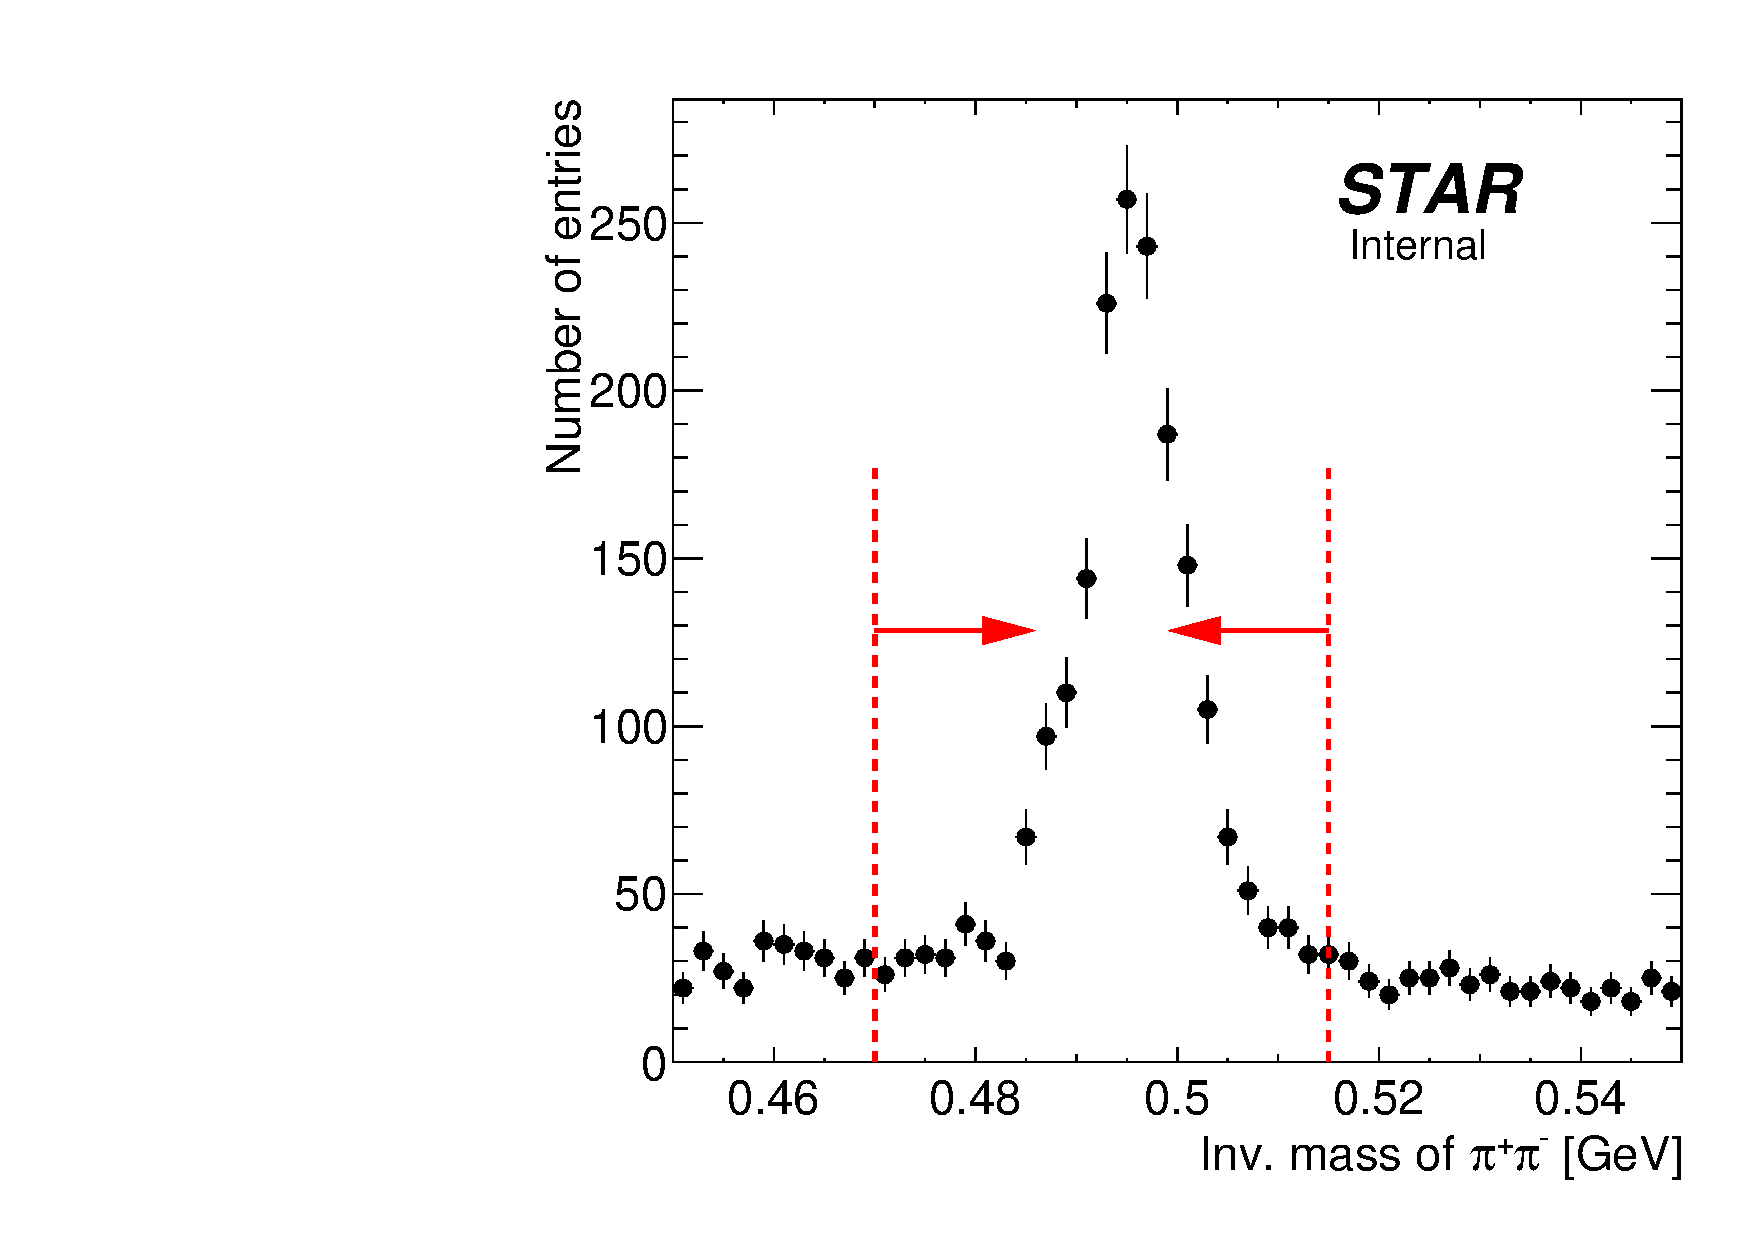
\includegraphics[width=\linewidth]{graphics/deadMaterial/InvMassAssumingPiPlusPiMinus.pdf}\vspace{-6pt}}}
  \end{subfigure}
} 
\quad
\parbox{0.31\textwidth}{
  \centering
  \begin{subfigure}[b]{\linewidth}{
                \subcaptionbox{\label{fig:invMassLambda}}{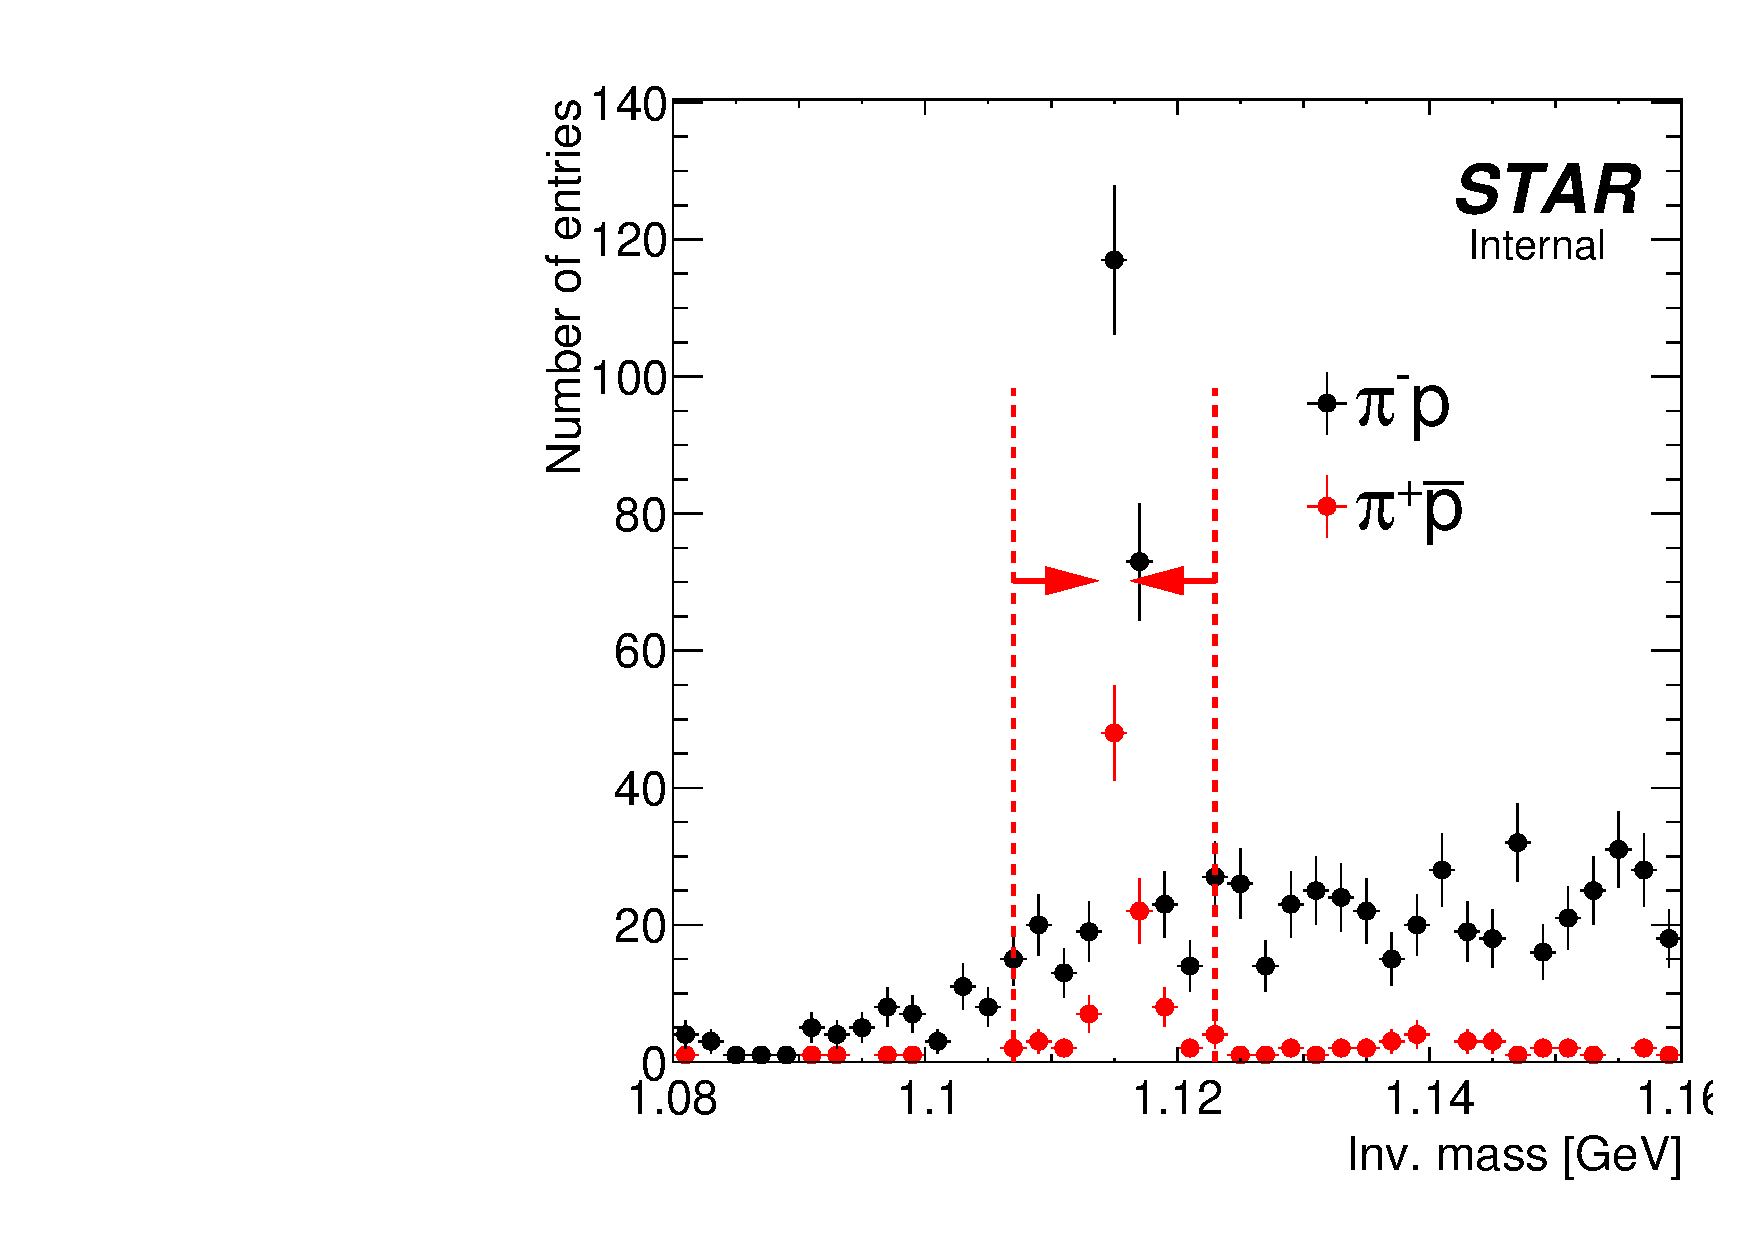
\includegraphics[width=\linewidth]{graphics/deadMaterial/InvMassLambdaSearch.pdf}\vspace{-6pt}}}
  \end{subfigure}
}
\quad
\parbox{0.31\textwidth}{
  \centering
  \begin{subfigure}[b]{\linewidth}{
                \subcaptionbox{\label{fig:cosThetaEPlusEMinus}}{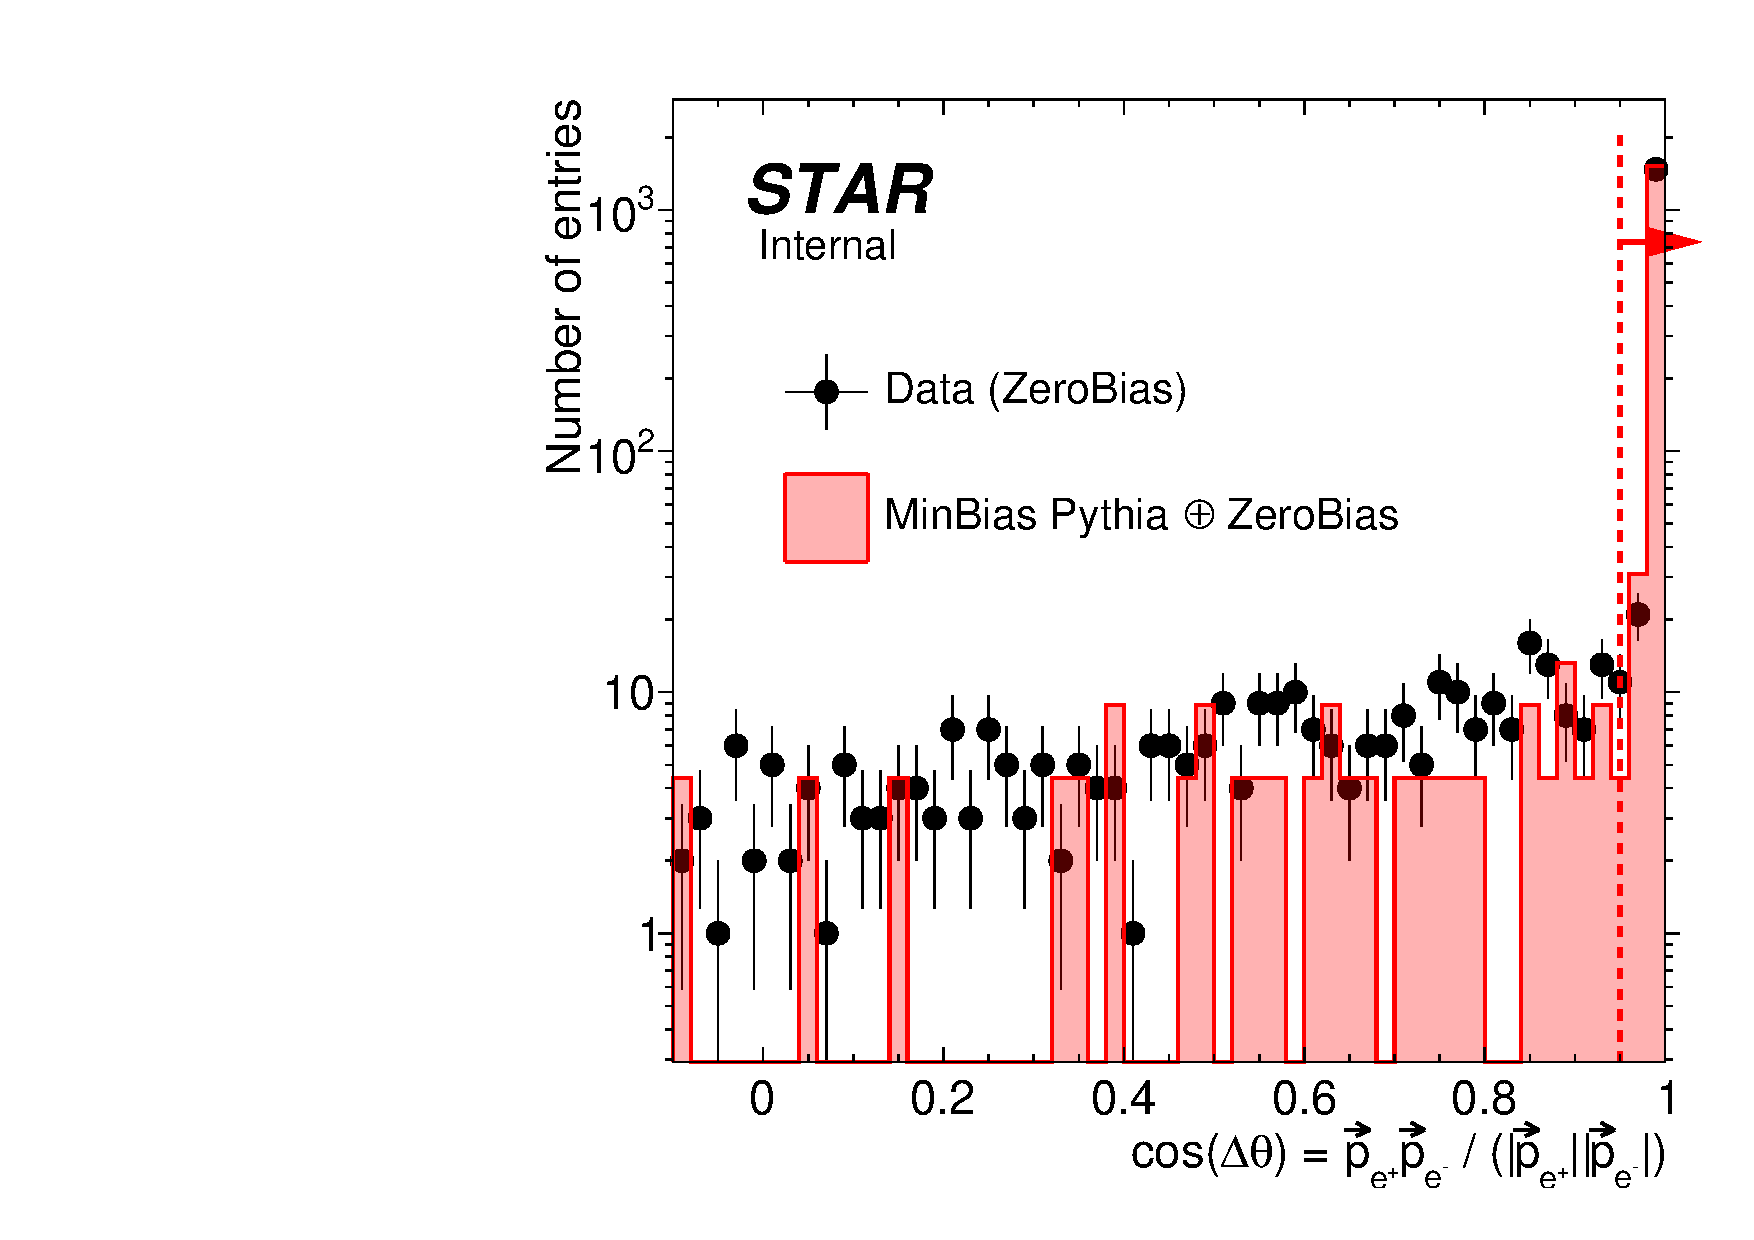
\includegraphics[width=\linewidth]{graphics/deadMaterial/CosDeltaThetaEPlusEMinus.pdf}\vspace{-6pt}}}
  \end{subfigure}
}\vspace{-4pt}
\caption[Invariant mass of two opposite-sign tracks and cosine of the opening angle between tracks forming a secondary vertex.]%
    {Invariant mass of two opposite-sign tracks recognized as $\pi^{+}\pi^{-}$ (\ref{fig:invMassK0S}) and $\pi^{+}\bar{p}$/$\pi^{-}p$ pair (\ref{fig:invMassLambda}), and cosine of the opening angle between two opposite-sign tracks recognized as $e^{+}e^{-}$ pair (\ref{fig:cosThetaEPlusEMinus}), forming a secondary vertex. Dashed red lines and red arrows indicate ranges of quantities which define particular nature of the secondary vertex (photoconversion/resonance decay/hadronic). All three plots represent zero-bias data.}\label{fig:secVtxTypeSelection}\vspace{-20pt}%
\end{figure}
%---------------------------

After secondary track candidates were selected, the following algorithm for secondary vertex reconstruction was used:%\\[-20pt]%
\vspace{-6pt}\begin{enumerate}
    \item Loop over all pairs of secondary track candidates, store pairs whose DCA is less than 0.5~cm (nearby tracks passing a proximity cut),\vspace{-6pt}
    \item Link pairs of nearby tracks into sets of tracks connected by the common nearby tracks,\vspace{-6pt}
    \item Loop over all sets defined in 2., in each set loop over all pairs from given set, reject worst-matching tracks (these with largest DCA to others) until all pairs of tracks have DCA less than 0.5~cm,\vspace{-6pt}
    \item Based on number of tracks in secondary vertex, total charge, specific energy loss, $dE/dx$, cosine of the opening angle of two tracks $cos(\Delta\theta)$ and invariant mass of two tracks $m_{\text{inv}}$ determine if the vertex is from resonance decay, photoconversion or is of nuclear/hadronic nature:\\[-16pt]
    \begin{enumerate}
    \item if $\geq2$ tracks in the vertex, or 2 tracks of the same sign, or 2 tracks of the opposite sign and cosine of the opening angle between two tracks $cos(\Delta\theta)<-0.99$ (tracks back-to-back) vertex is recognized as hadronic; otherwise (sub-sample of 2 opposite-sign tracks case remains)\\[-15pt]
    \item if $|n^{\sigma}_{\text{pion}}|<3$ for both tracks and invariant mass (assuming pion mass) is within $[0.470,0.515]$~GeV (Fig.~\ref{fig:invMassK0S}) the vertex is recognized as originating from the decay of $K^{0}_{S}$; otherwise\\[-15pt]
    \item if $|n^{\sigma}_{\text{pion}}|<3$ for one track and $|n^{\sigma}_{\text{proton}}|<3$ for the other, and invariant mass (assuming pion and proton mass, respectively) is within $[1.107,1.123]$~GeV (Fig.~\ref{fig:invMassLambda}) the vertex is recognized as originating from the $\Lambda$/$\bar{\Lambda}$ decay; otherwise\\[-15pt]
    \item if $|n^{\sigma}_{\text{electron}}|<3$ for both tracks and invariant mass (assuming electron mass) is less than $0.09$~GeV and cosine of the opening angle between two tracks $cos(\Delta\theta)>0.95$ (Fig.~\ref{fig:cosThetaEPlusEMinus}) the vertex is recognized as originating from photoconversion; otherwise the vertex is recognized as hadronic.
    \end{enumerate}%
\end{enumerate}%
~
\begin{enumerate}[resume, before = \vspace*{-23pt}]
 \item Calculate the vertex position as the average DCA point of all track pairs in the vertex.
\end{enumerate}




%---------------------------
\begin{figure}[t!]\vspace{-2pt}%
\centering%
\begin{minipage}{.4725\textwidth}%
  \centering%
  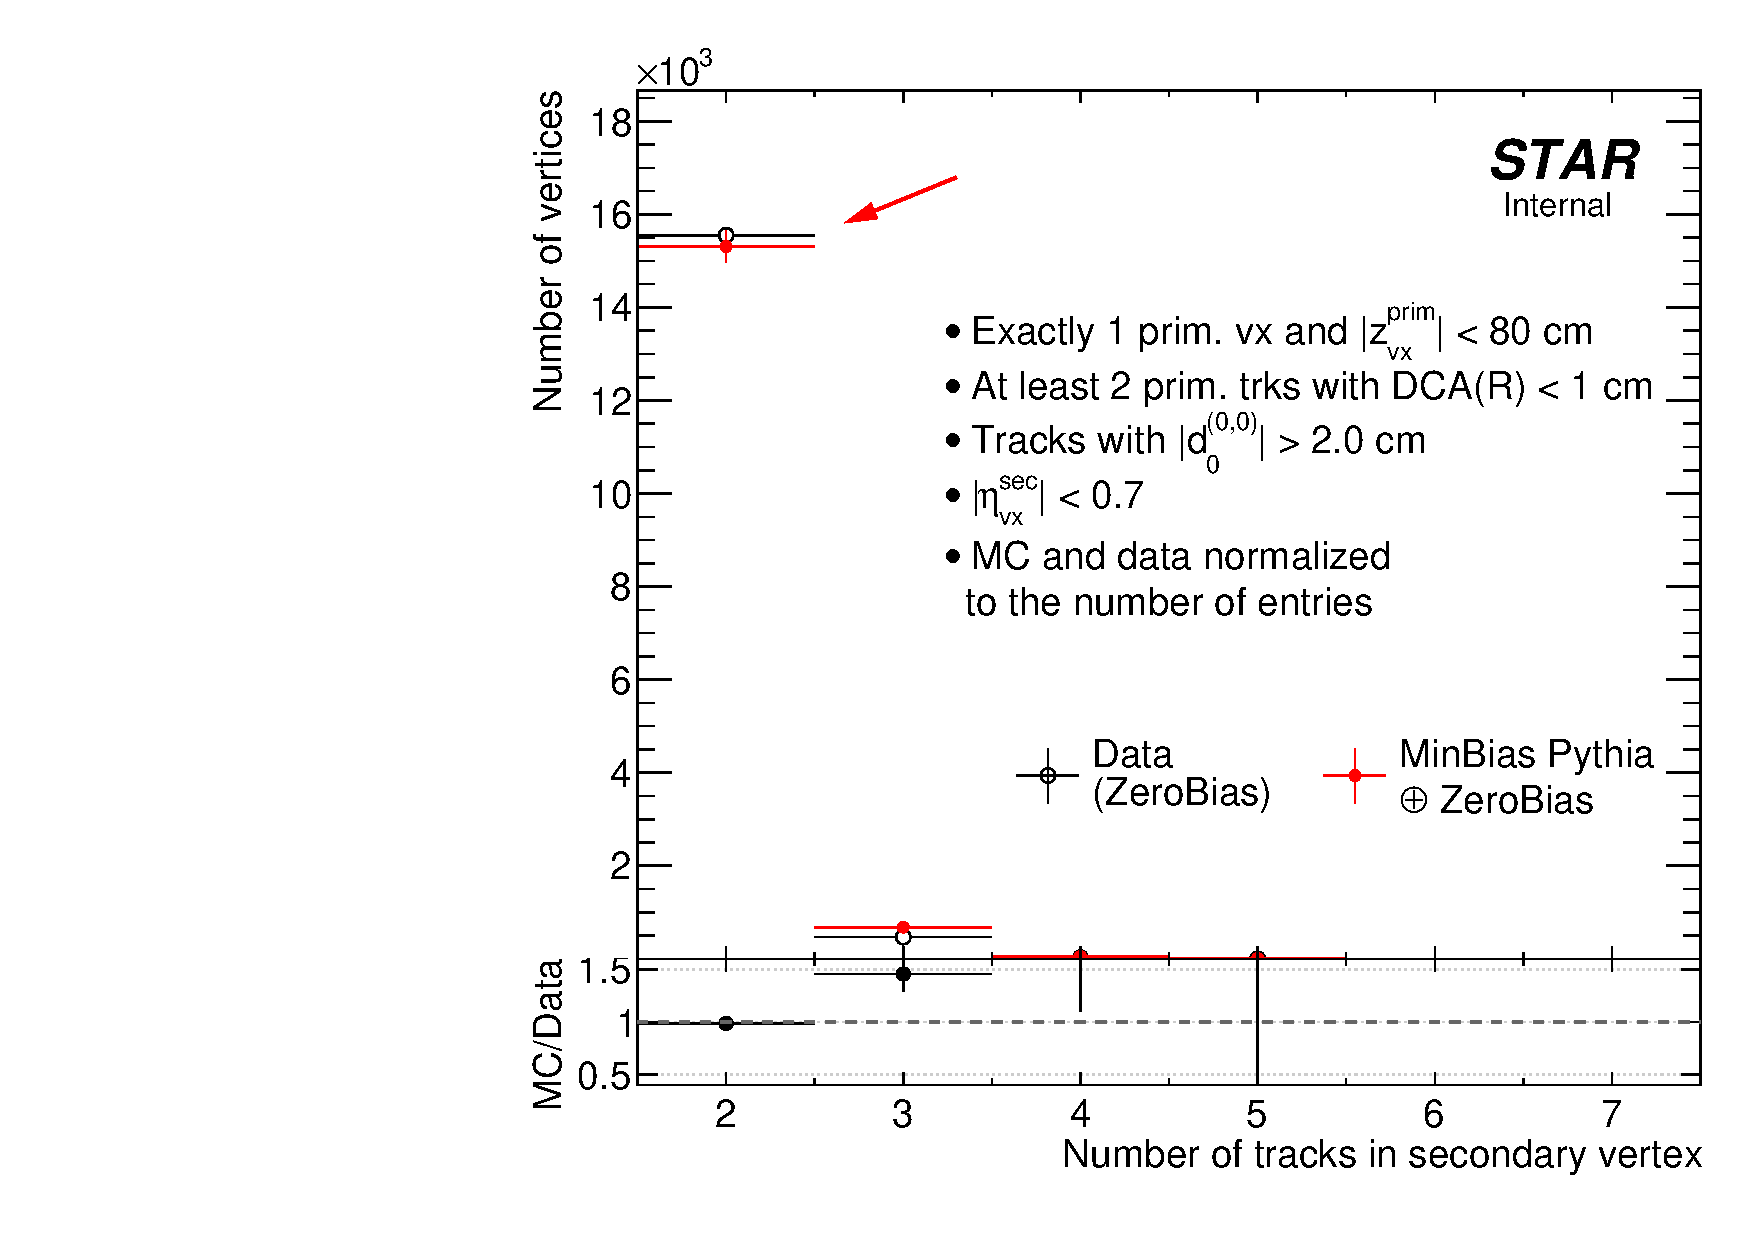
\includegraphics[width=\linewidth]{graphics/deadMaterial/NTracksInVertex_DataVsMC.pdf}%\vspace*{-10pt}%
  \caption[Multiplicity of tracks in reconstructed secondary vertices.]{Multiplicity of tracks in reconstructed secondary vertices. Red arrow points to bin with vertices used in final analyses of vertex distribution.}\label{fig:nTrksInSecVx}
\end{minipage}%
\quad\quad%
\begin{minipage}{.4725\textwidth}%
  \centering
  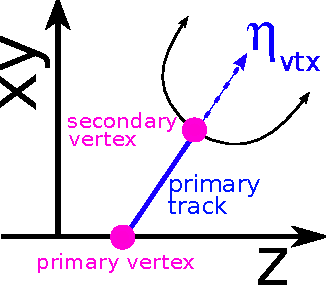
\includegraphics[width=0.9\linewidth]{graphics/deadMaterial/etaVxCut2.pdf}\vspace*{ 15pt}
  \caption[$\eta_{\text{vtx}}$ definition (sketch).]{$\eta_{\text{vtx}}$ definition (sketch).}%
   \label{fig:etaVxCut}
\end{minipage}%
\end{figure}%
%---------------------------

%---------------------------
\begin{figure}[b!]\vspace{-10pt}
\centering
\parbox{0.4725\textwidth}{
  \centering
  \begin{subfigure}[b]{\linewidth}
                \subcaptionbox{\label{fig:RVertex_DataVsMC}}{\includegraphics[width=\linewidth,page=3]{graphics/deadMaterial/RVertex_DataVsMC.pdf}\vspace{-15pt}}
  \end{subfigure}
}%
\quad\quad%
\parbox{0.4725\textwidth}{
  \centering
  \begin{subfigure}[b]{\linewidth}
                \subcaptionbox{\label{fig:ZVertex_DataVsMC}}{\includegraphics[width=\linewidth,page=3]{graphics/deadMaterial/ZVertex_DataVsMC.pdf}\vspace{-15pt}}
  \end{subfigure}
}\vspace{-5pt}%
\caption[Comparison of raw $R_{\text{vtx}}^{\text{secondary}}$ and $z_{\text{vtx}}^{\text{secondary}}$ distribution in the data and embedded MC.]%
{Comparison of raw $R_{\text{vtx}}^{\text{secondary}}$ (\ref{fig:RVertex_DataVsMC}) and $z_{\text{vtx}}^{\text{secondary}}$ (\ref{fig:ZVertex_DataVsMC}) distribution in the data (opened black circles) and embedded MC (filled red circles). Only vertices recognized as products of hadronic interactions are shown in the figure. Solid lines denote estimated backgroud content in the distribution of corresponding color.}\vspace{-10pt}\label{fig:RZVertexDataVsMC}%
\end{figure}
%---------------------------

As a result secondary vertices were reconstructed, whose track multiplicity distribution is depicted in Fig.~\ref{fig:nTrksInSecVx}. Analysis was continued only with vertices of multiplicity equal 2. The first reason was that most of vertices consist of just a pair of tracks. Another reason was the background subtraction method developed only for vertices made of two tracks. In addition to this, only vertices representing primary particles in the pseudorapidity range $-0.7 < \eta < 0.7$ were analyzed. To enable such selection a variable $\eta_{\text{vtx}}$ was defined, as shown in Fig.~\ref{fig:etaVxCut}.

Raw distributions of $R_{\text{vtx}}^{\text{secondary}}$ and $z_{\text{vtx}}^{\text{secondary}}$ are shown in Fig.~\ref{fig:RVertex_DataVsMC} and Fig.~\ref{fig:ZVertex_DataVsMC}, respectively. In $R_{\text{vtx}}^{\text{secondary}}$ spectrum one can find peaks in the regions where the HFT subdetectors are placed. Peaks seem to lie on top of a tail whose origin has been identified with the secondary vertices made of pair of tracks, one of which was a true primary tracks that was not associated with any primary vertex and unfortunately passed selection of global tracks for the secondary vertex reconstruction. For this reason a method of estimation of the backgroud was invented, as described in the next paragraph. Without this backgroud subtracted, the ratio of MC to data varies mostly between 0.5 and 0.7.

Background estimation makes use of different content of fake secondary vertices depending on the proximity cut used in the secondary vertex reconstruction. This method is enabled by good agreement of the shape of the tails in distributions of the DCA between two tracks forming a secondary vertex in data and MC, as shown in Figure~\ref{fig:DcaOfTwoGlobalTofTrksWithLargeD0_DataVsMC}. %
%
%---------------------------
\begin{figure}[t!]\vspace{-2pt}%
\centering%
\begin{minipage}{.4725\textwidth}%
  \centering%\vspace{11pt}
  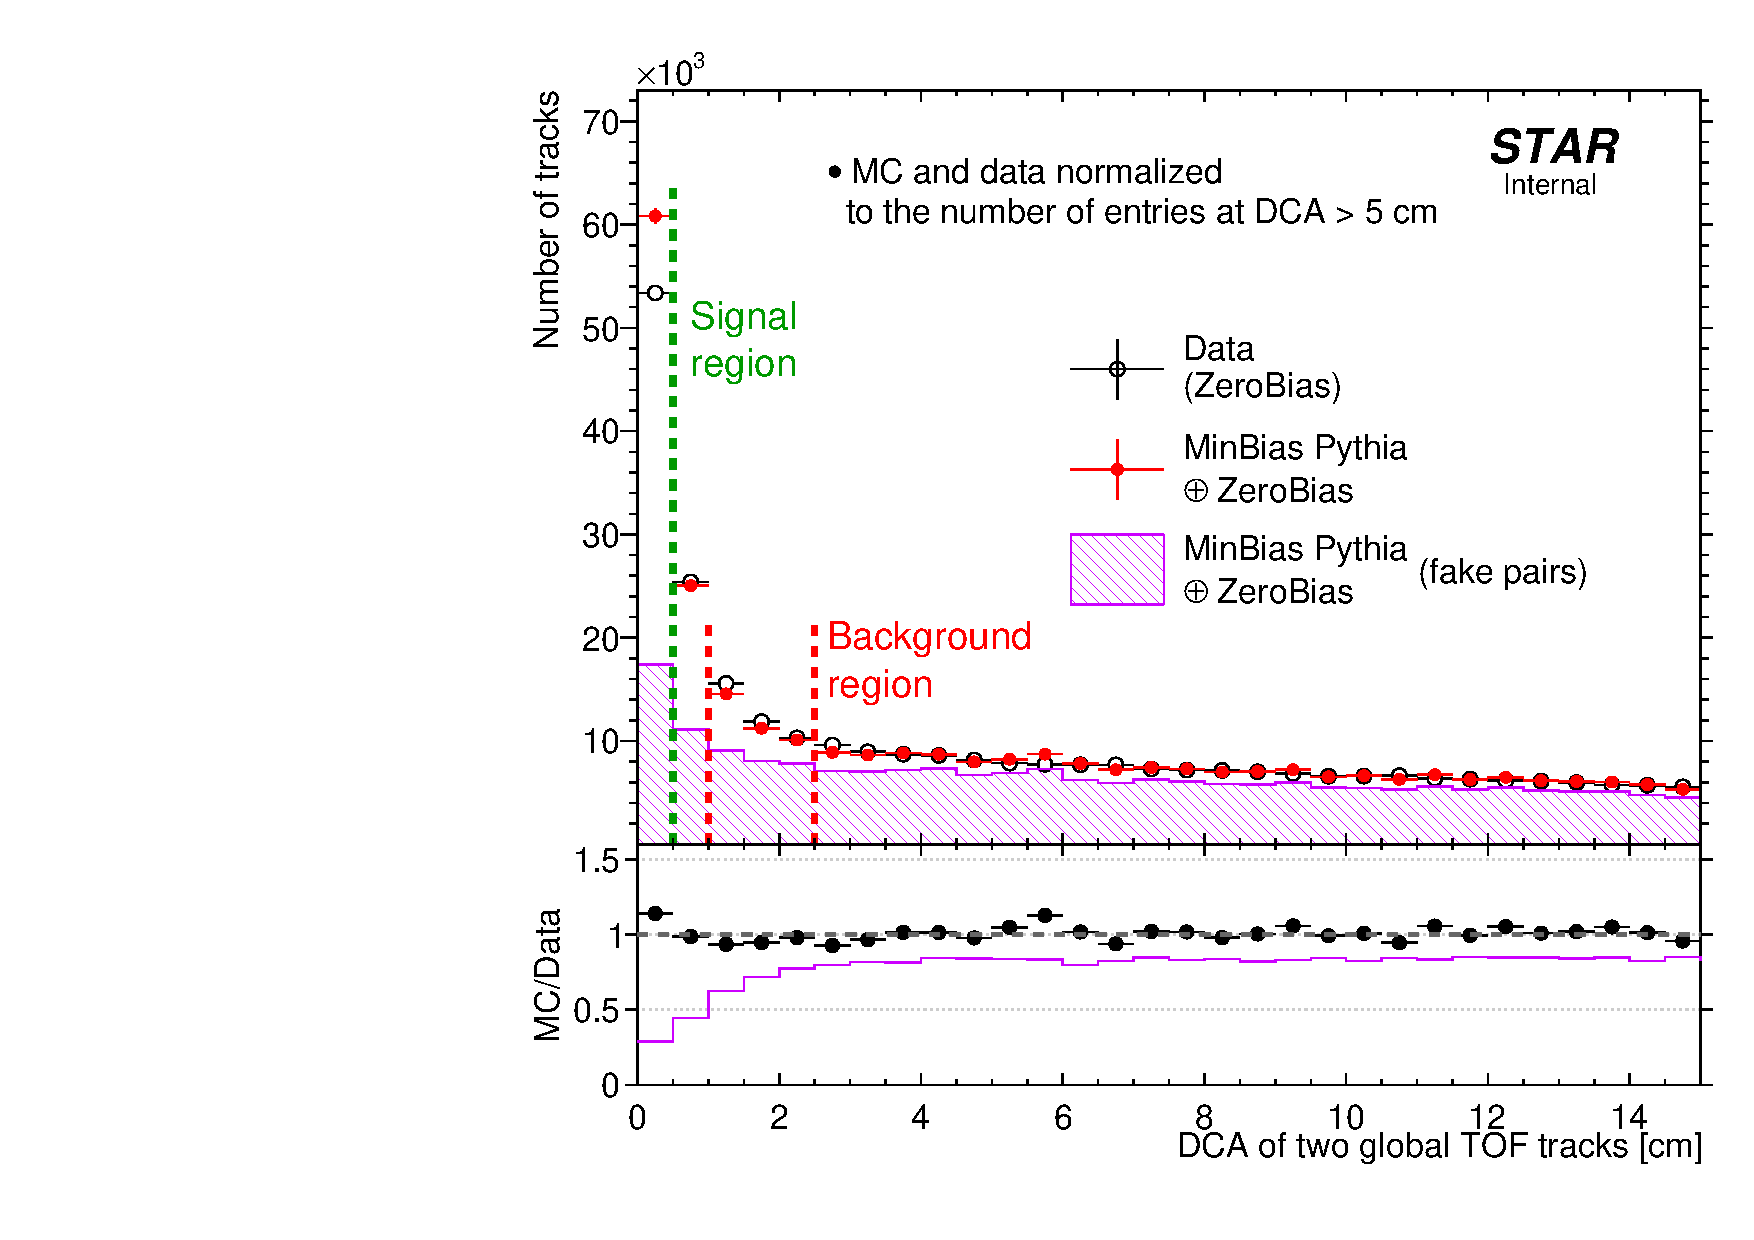
\includegraphics[width=\linewidth]{graphics/deadMaterial/DcaOfTwoGlobalTofTrksWithLargeD0_DataVsMC.pdf}\vspace{-5pt}%
  \caption[Comparison of DCA between all pairs of secondary track candidates selected for the secondary vertex reconstruction in the data and embedded MC.]%
  {Comparison of DCA between all pairs of secondary track candidates selected for the secondary vertex reconstruction  in the data and embedded MC. MC histogram is normalized to the data at $\text{DCA}>5$~cm. Violet hashed histogram depicts pairs contained in MC histogram and not originating from the same vertex. Solid violet line in the lower pad denotes ratio of violet and red histogram.\newline\newline }\label{fig:DcaOfTwoGlobalTofTrksWithLargeD0_DataVsMC}
\end{minipage}%
\quad\quad%
\begin{minipage}{.4725\textwidth}%
  \centering%
  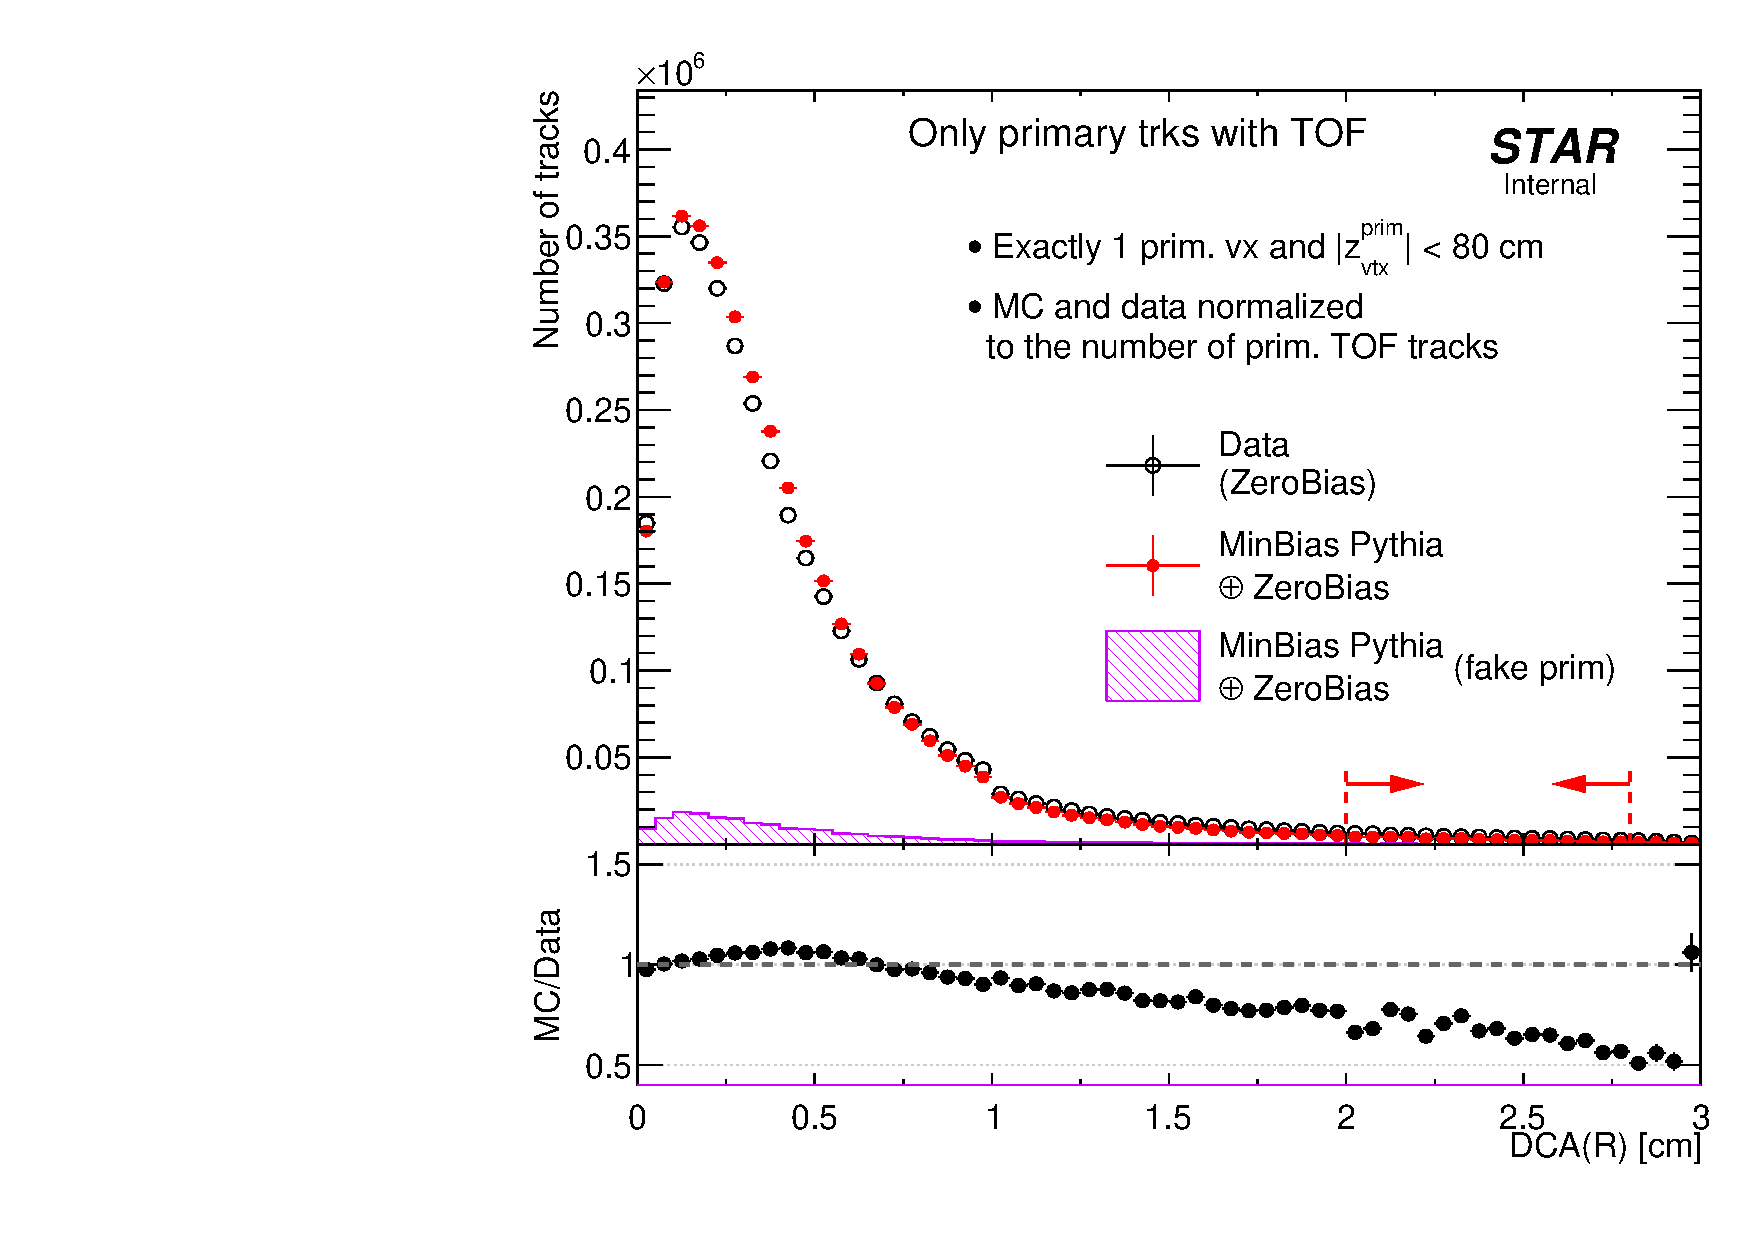
\includegraphics[width=\linewidth]{graphics/deadMaterial/DcaRPrimary_Tof_SelectedEvents_DataVsMC.pdf}\vspace*{-5pt}
  \caption[Comparison of radial DCA of all primary tracks matched with TOF and passing quality criteria in events selected for secondary vertex analysis, between the data and embedded MC.]
   {Comparison of radial DCA of all primary tracks matched with TOF and passing quality criteria in events selected for secondary vertex analysis, between the data and embedded MC. Violet hashed histogram represents tracks not matched to true-level particles. Red dashed lines and arrows limit region used to find normalization that compensates different backgroud yield in reconstructed secondary vertex distributions in data and embedded MC. Discontinuity at 1~cm is due to selection of events with at least 2 tracks of $\text{DCA}(\text{R})<1~\text{cm}$}
   \label{fig:primaryDcaSelectedEvtsDataVsMC}%\vspace*{-29pt}
\end{minipage}\vspace{-12pt}%
\end{figure}%
%---------------------------
%
The most optimal cut to select pairs from the secondary vertices is as low as about 0.5~cm, however one can change the proximity cut to form vertices from tracks of DCA within some higher limits, which results in different ratio of signal to background vertices. In Fig.~\ref{fig:DcaOfTwoGlobalTofTrksWithLargeD0_DataVsMC} the nominal proximity cut is marked with the green line (signal region), while the modified proximity cut is marked with red lines (backgroud region). With such two versions of cuts used in vertexing the two independent distributions of secondary vertices can be obtained: one with the standard proximity cut - $\mathcal{H}_{1}$, the other with modified proximity cut, in our case $1.0~\text{cm}<\text{DCA}<2.5~\text{cm}$ - $\mathcal{H}_{2}$. Limits in modified proximity cut were set to such values in order to ensure similar statistics in signal and backgroud region, as well as provide the same (very similar) resolution of secondary vertex position calculated as a middle point between DCA points on helices associated with the tracks. One can note that the content of histograms (normalized to the same number of entries, $\int\mathcal{H}_{2}=\int\mathcal{H}_{1}$) can be described by the set of equations given below:\vspace*{-4pt}
   \begin{empheq}[left=\empheqlbrace]{align}
     \mathcal{H}_{1} &= (1-\kappa B)\times signal~ + \kappa B\times background,\label{eq:h1} \\
     \mathcal{H}_{2} &= (1-\kappa B')\times signal + \kappa B'\times background,\label{eq:h2}
   \end{empheq}%
in which parameters $B$ and $B'$ ($B \neq B'$) denote the fraction of fake secondary vertices in the distribution resultant from analysis utilizing nominal and modified proximity cut, respectively, and $signal$ and $backgroud$ denote distributions of only true and only fake secondary vertices, respectively. Meaning of the $\kappa$ parameter (equal to 1 for the time being) is explained in the next paragraph. The solution to set of Eqs.~\eqref{eq:h1},~\eqref{eq:h2} is the following:
   \begin{empheq}[left=\empheqlbrace]{align}
     signal &= \frac{B'\times \mathcal{H}_{1} - B\times \mathcal{H}_{2}}{B'-B}\label{eq:signal} \\
     background &= \frac{(1-\kappa B)\times \mathcal{H}_{2} - (1-\kappa B')\times \mathcal{H}_{1}}{\kappa (B'-B)}\label{eq:bkgd}
   \end{empheq}%
An important remark here is that the backgroud fraction extracted from the ratio of violet and red histograms in Fig.~\ref{fig:DcaOfTwoGlobalTofTrksWithLargeD0_DataVsMC} can be used directly in Eqs.~\eqref{eq:h1}-\eqref{eq:bkgd} only for backgroud estimation in MC. In other words, parameter $\kappa$ is equal to 1 only when solving Eqs.~\eqref{eq:signal}-\eqref{eq:bkgd} for MC. In case of background estimation in data parameters $B$ and $B'$ have to be corrected for the ``leakage'' of true primary tracks to set of selected secondary track candidates due to worse TPC track pointing resolution in the data, and thus lower probability/efficiency of attaching the true primary tracks to primary vertices at large DCA(R), as it was decribed in one of preceding paragraphs. The correction factor $\kappa$ is extracted from the ratio of the radial DCA of the primary TPC tracks in events selected for the secondary vertex study (Fig.~\ref{fig:primaryDcaSelectedEvtsDataVsMC}). This ratio at large DCA(R) provides estimate of how many more true primary TPC tracks in the data is not recognized as primary tracks (comparing to MC) and hence overpopulate/enrich sample of global tracks which are selected for the reconstruction of secondary vertices, by definition increasing number of fake, background secondary vertices. Histogram range selected for calculation of the ratio was set to $2.0~\text{cm}<\text{DCA}(R)<2.6~\text{cm}$, as this range coincides with the $d_{0}^{(0,0)}$ of global tracks accepted for the analysis ($d_{0}^{(0,0)}>2~\text{cm}$). $\kappa$ calculated in this range equals 1.5. It is clear from Fig.~\ref{fig:primaryDcaSelectedEvtsDataVsMC} that value of $\kappa$ depends on the limits of DCA(R) selected for the ratio calculation, therefore we determined and subtracted the backround using also values 1.2 and 1.8, which are the extreme cases in the bottom pad of aforementioned plot. In case $\kappa B$ or $\kappa B'$ exceeded 1, the unity was set to the product. The difference between these results and results for nominal $\kappa=1.5$ are considered as a systematic uncertainty of the number of secondary vertices.

Backgroud determined with the described method is shown in Fig.~\ref{fig:deadMatDataVsMC} with the solid lines colored according to corresponding markers (for nominal $\kappa$). This backgroud was subtracted and resulting distributions of the secondary vertex positions in the transverse and longitudinal direction are presented in Fig.~\ref{fig:RZVertexDataVsMC_BkgdSubtr}. Gray boxes represent systematic uncertainty on number of secondary vertices in the data due to $\kappa$ parameter uncertainty. Most releveant region - the HFT detector extending between $\sim$2~cm and $\sim$30~cm is satisfactorily well described by MC. Also, the inner wall of the TPC at $\sim$48~cm well matches between data and MC. Looking at the ratios in the bottom panels of Figs.~\ref{fig:deadMatDataVsMC} one can conclude that the differences between the dead material density in the data and STAR simulation generally vary between $\pm25\%$, which we consider a systematic uncertainty on the amount of the dead material in front of TPC. Related systematic uncertainty on the TPC track reconstruction efficiency is described in Sec.~\ref{sec:deadMaterialSystematics}.



%---------------------------
\begin{figure}[hb]
\centering
\parbox{0.4725\textwidth}{
  \centering
  \begin{subfigure}[b]{\linewidth}
                \subcaptionbox{\label{fig:RVertex_DataVsMC_BkgdSubtr}}{\includegraphics[width=\linewidth,page=3]{graphics/deadMaterial/RVertex_BackgroudSubtracted_DataVsMC.pdf}}\vspace{-5pt}
  \end{subfigure}
}%
\quad\quad%
\parbox{0.4725\textwidth}{
  \centering
  \begin{subfigure}[b]{\linewidth}
                \subcaptionbox{\label{fig:ZVertex_DataVsMC_BkgdSubtr}}{\includegraphics[width=\linewidth,page=3]{graphics/deadMaterial/ZVertex_BackgroudSubtracted_DataVsMC.pdf}}\vspace{-5pt}
  \end{subfigure}
}%
\caption[Comparison of background-subtracted $R_{\text{vtx}}^{\text{secondary}}$ and $z_{\text{vtx}}^{\text{secondary}}$ distribution in the data and embedded MC.]% 
    {Comparison of background-subtracted $R_{\text{vtx}}^{\text{secondary}}$ (\ref{fig:RVertex_DataVsMC_BkgdSubtr}) and $z_{\text{vtx}}^{\text{secondary}}$ (\ref{fig:ZVertex_DataVsMC_BkgdSubtr}) distribution in the data (opened black circles) and embedded MC (filled red circles). Only vertices recognized as products of hadronic interactions are shown in the figure.}\label{fig:RZVertexDataVsMC_BkgdSubtr}%
\end{figure}
%---------------------------
